% PLANTILLA APA7
% Creado por: Isaac Palma Medina
% Última actualización: 25/07/2021
% @COPYLEFT

% Fuentes consultadas (todos los derechos reservados):  
% Normas APA. (2019). Guía Normas APA. https://normas-apa.org/wp-content/uploads/Guia-Normas-APA-7ma-edicion.pdf
% Tecnológico de Costa Rica [Richmond]. (2020, 16 abril). LaTeX desde cero con Overleaf (1 de 3) [Vídeo]. YouTube. https://www.youtube.com/watch?v=kM1KvHVuaTY Weiss, D. (2021). 
% Formatting documents in APA style (7th Edition) with the apa7 LATEX class. https://ctan.math.washington.edu/tex-archive/macros/latex/contrib/apa7/apa7.pdf @COPYLEFT

%+-+-+-+-++-+-+-+-+-+-+-+-+-++-+-+-+-+-+-+-+-+-+-+-+-+-+-+-+-+-++-+-+-+-+-+-+-+-+-+

% Preámbulo
\documentclass[stu, 12pt, letterpaper, donotrepeattitle, floatsintext, natbib, helv]{apa7}
\usepackage{listings}
\usepackage[utf8]{inputenc}
\usepackage{comment}
\usepackage{marvosym}
\usepackage{graphicx}
\usepackage{float}
\usepackage[normalem]{ulem}
\usepackage[spanish]{babel} 
%\usepackage{titling}
\let\apasubparagraph\subparagraph
\let\subparagraph\paragraph
\usepackage[compact]{titlesec}
\let\subparagraph\apasubparagraph
\usepackage{hyperref}
\selectlanguage{spanish}
\useunder{\uline}{\ul}{}
\newcommand{\myparagraph}[1]{\paragraph{#1}\mbox{}\\}
\graphicspath{{./Images/}}
\titleformat{\section}{\normalfont\large\bfseries}{\thetitle. \quad }{0pt}{}[{ \titlerule[0.8pt]}]
\titleformat{\subsection}{\normalfont\bfseries}{}{}{}[]

% Portada

\begin{document}
\begin{titlepage}
    \centering
    \vfill
    \LARGE Análisis de métodos de buscar\\
    \vskip2cm
    \large Diego Quirós Artiñano \\
    Universidad Nacional de Costa Rica \\
    EIF-203: Estructuras Discretas (10 A.M.) \\ 
    Carlos Loria-Saenz \\
    24 de marzo, 2022 \\
    \vfill
    
\includegraphics[width = 0.4\textwidth]{/home/xarthy/UNAImage/UNA.png} \\
    \vfill
    \vfill
    % (autores separados, consultar al docente)
    % Manera oficial de colocar los autores:
    %\author{Autor(a) I, Autor(a) II, Autor(a) III, Autor(a) X}
\end{titlepage}

% Índices
\pagenumbering{roman}
    % Contenido
\renewcommand\contentsname{\largeÍndice}
\tableofcontents
\setcounter{tocdepth}{2}
\newpage
    % Figuras
\renewcommand{\listfigurename}{\largeÍndice de fíguras}
\listoffigures
\newpage
    % Tablas
\renewcommand{\listtablename}{\largeÍndice de tablas}
\listoftables
\newpage

% Cuerpo
\pagenumbering{arabic}

%------------------------------------------------------------------------------------
\section{Análisis de es\_simetrica()}
\begin{enumerate}
    \setcounter{enumi}{-1}
    \item El algoritmo original.
\end{enumerate}
\begin{lstlisting}[language=Python]
    def es_simetrica(a:list[list[int]])-> bool:
        for i in range(len(a)):
            for j in range(i+1, len(a[i])):
                if i != j and a[i][j] != a[j][i]:
                    return False
        return True
\end{lstlisting}
\begin{enumerate}
    \setcounter{enumi}{0}
    \item Tamaño de los datos \\
El método se construyó de manera en la que no busque la diagonal de la matriz y solo se tiene que buscar la parte de arriba, entonces el tamaño de datos es $frac{n(n-1)}{2}$
    \item Operaciones de Interés \\
    \begin{table}[h]
        \centering
        \begin{tabular}{|c c c|} 
         \hline
         Notación [en función de tiempo (T)] & Operación & Tipo de Operación \\ [0.5ex] 
         \hline\hline
         $T_{range()}$ & range(len(a)) or range(i+1, len(a[i])) & constante \\ 
         \hline
         $T_{!=}$ & i != j or a[i][j] != a[j][i] & constante \\
         \hline
         $T_{[]}$ & a[i][j] or a[j][i] & constante [1ex]
         \hline
        \end{tabular}
        \caption{Operaciones es\_simetrica()}
        \label{tab:tablesimetrica}
    \end{table}
        Peor caso: toas son iguales a la mas grande de todas, como supuesto \\
        Asumimos que vale 1 (unidad de tiempo), según el más alto
    \item Ecuación
    \end{enumerate}
\begin{lstlisting}[language=Python]
    # Separando por partes
    # Parte 1
    p:int = 0
    # Parte 2
    while p < len(a):
        if x == a[p]:
            return p
        else:
            p += 1
    # Parte 3
    return -1
\end{lstlisting}

\[T_{buscar\_while()}(n) = T_{parte1} + T_{parte2} + T_{parte3} \] \\ 
\[T_{buscar\_while()}(n) = 1 + T_{while()}(n) + 0\] \\
\[T_{buscar\_while()}(n) = T_{while()}(n) + 1\] \\
Evaluando $T_{while()}(n)$: \\
2 operaciones: < y len(a) \\
2 operaciones: == y $[]$ \\
1 operación: +=

Entonces: \[T_{while()}(n) = 2 + 2 + 1 + T_{while()}(n-1)\] \\
\[T_{while()}(n) = 5 + 5 + 5 + ... T_{while()}(0)\] \\
Como el while va a verificar si sigue siendo parte del while entonces se cuentan las primeras 2 operaciones otra vez:
\[T_{while()}(N) = 5n + 2\]

\begin{enumerate}
    \setcounter{enumi}{3}
    \item Volviendo a meter en la ecuación original:
\[T_{buscar\_while()}(n) = 5n + 2 + 1\] \\
\[T_{buscar\_while()}(n) = 5n + 3\] \\
    \item Orden de crecimiento \\
Como la ecuación es una función lineal entonces el orden de crecimiento también lo cual significa que: $O(n) \sim T_{buscar_while()}(n)$
    \item Código
\end{enumerate}
\begin{lstlisting}[language=Python]
    def buscar_while_instrumentado(x:int, a:list[int])-> int:
        contador_operaciones = 0
        p:int = 0
        contador_operaciones += 1
        no_salir = p < len(a)
        contador_operaciones += 2
        while no_salir:
            if x == a[p]:
                contador_operaciones += 2
                return contador_operaciones
            else:
                contador_operaciones += 2
                p += 1
                contador_operaciones += 1
            no_salir = p < len(a)
            contador_operaciones += 2
        return contador_operaciones
\end{lstlisting}

\section{Excel}
Para importar a Excel para hacer la gráfica, se hizo este código:
{\scriptsize
\begin{lstlisting}[language=Python]
    def test_buscar_instrumentado(filename, init, maxi, inc):
        file = open(filename, 'w')
        file.write('n;time_while;time_for\n')
        for n in range(init, maxi, inc):
            a = list(range(n))
            x = n
            file.write(f'{n};{buscar_while_instrumentado(x,a)};{buscar_for_instrumentado(x,a)}\n')
        file.close()
    test_buscar_instrumentado('buscar_instrumentado.csv', 10, 200, 10)
\end{lstlisting}}

\begin{figure}[h]
    \centering
    %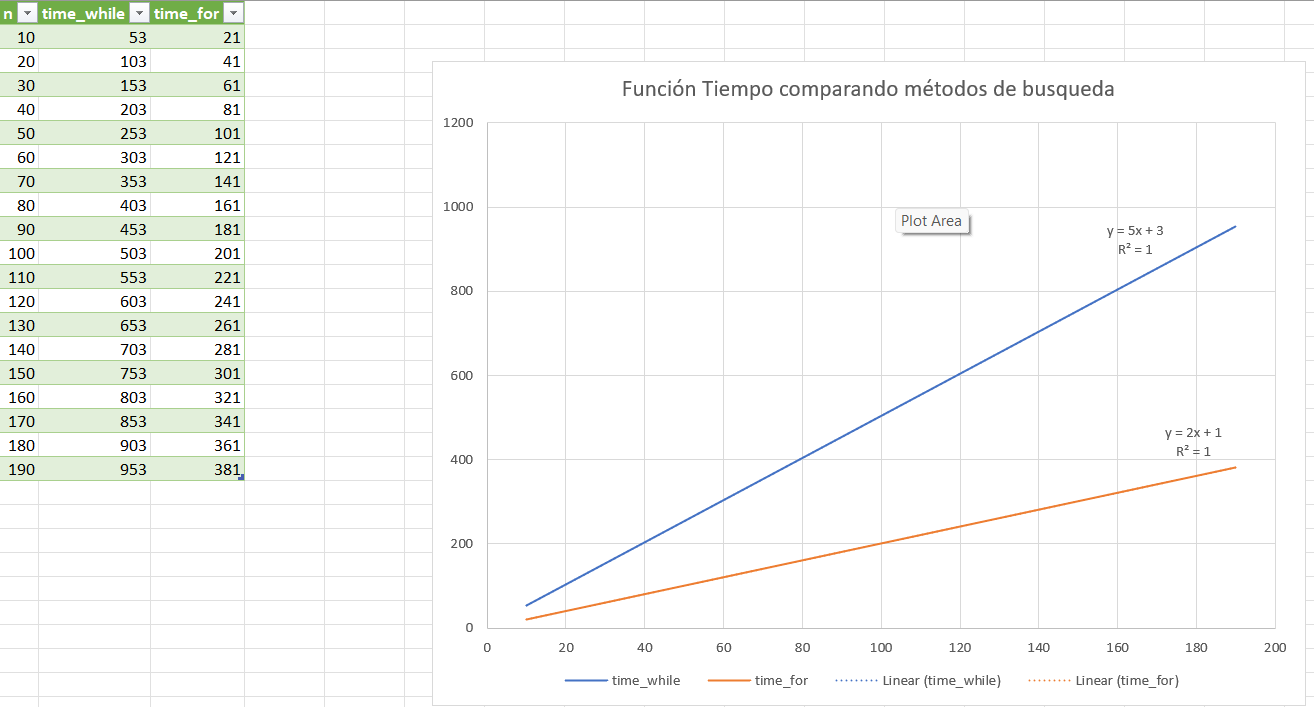
\includegraphics[width=1.2\textwidth]{CroppedExcelGraph.png}
    \caption{Gráfica de los métodos en Excel}
    \label{fig:figureExcel1}
\end{figure}
\nocite{Clase21Mar}
\newpage
\renewcommand\refname{\large\textbf{Referencias}}
\bibliography{ref}

\end{document}